\subsection{Computational cost}
\label{app:computational-cost-flops}
In the scaling experiments (Sections \ref{sec:scaling_results} and \ref{sec:results_task_scaling}), we compare agents after they have been trained for an equivalent number of steps. While this controls for sample efficiency of models, here we provide an analysis of the computational cost in FLOPs for a given experiment, and reproduce some of our scaling results, controlling for for compute cost. We see that bigger is not always better from this perspective. 
For each model size and memory length we use JAX \citep{jax2018github} cost analysis to estimate the number of FLOPs per frame of the learner step and actor step (Table \ref{tab:flops}).

\begin{figure}[t!]
    \centering
    \begin{subfigure}[b]{0.49\textwidth}
        \centering
        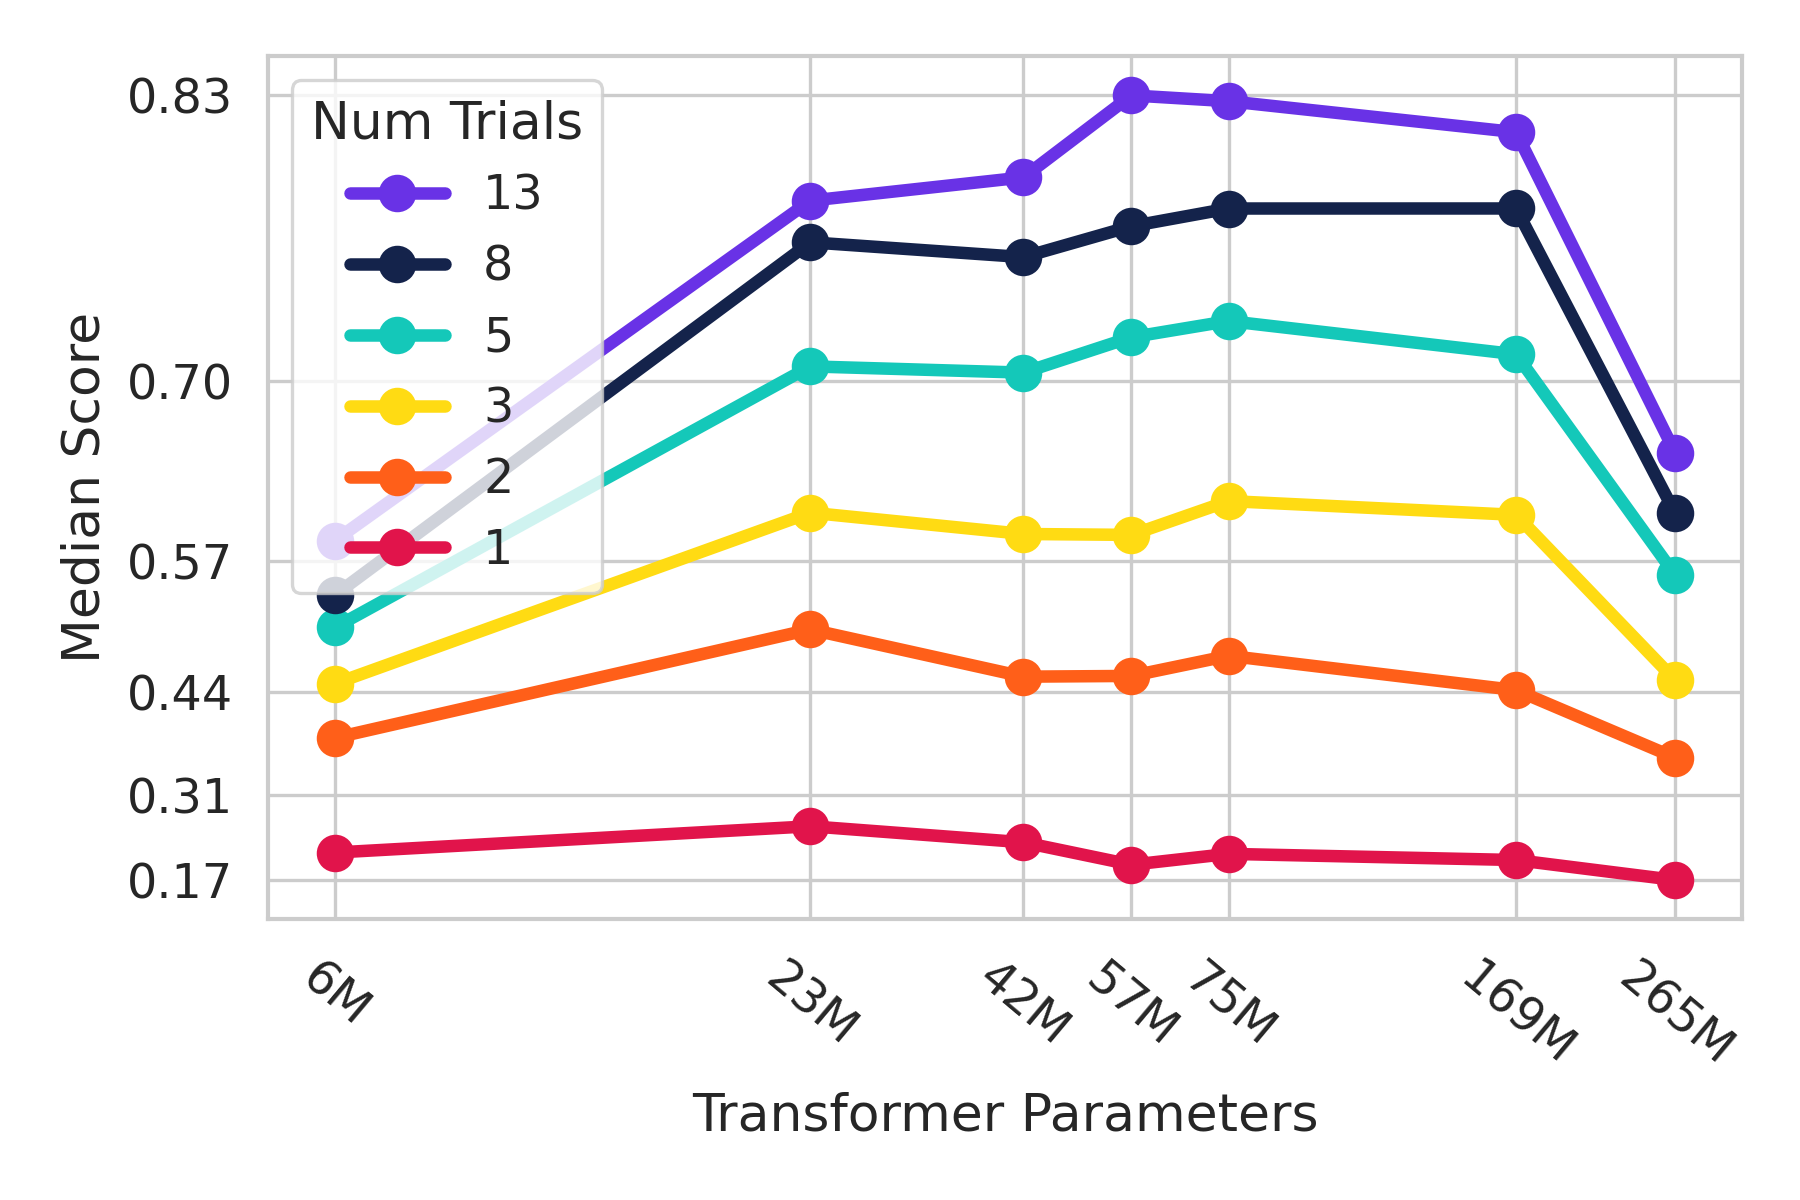
\includegraphics[width=\linewidth]{figures/scaling_flops/parameter_scaling_total_flops_percentile50_log_log.png}
        \vskip -3pt \caption{}
    \label{figure:scaling_parameters_total_flops_50th}
    \end{subfigure}
    \begin{subfigure}[b]{0.49\textwidth}
        \centering
        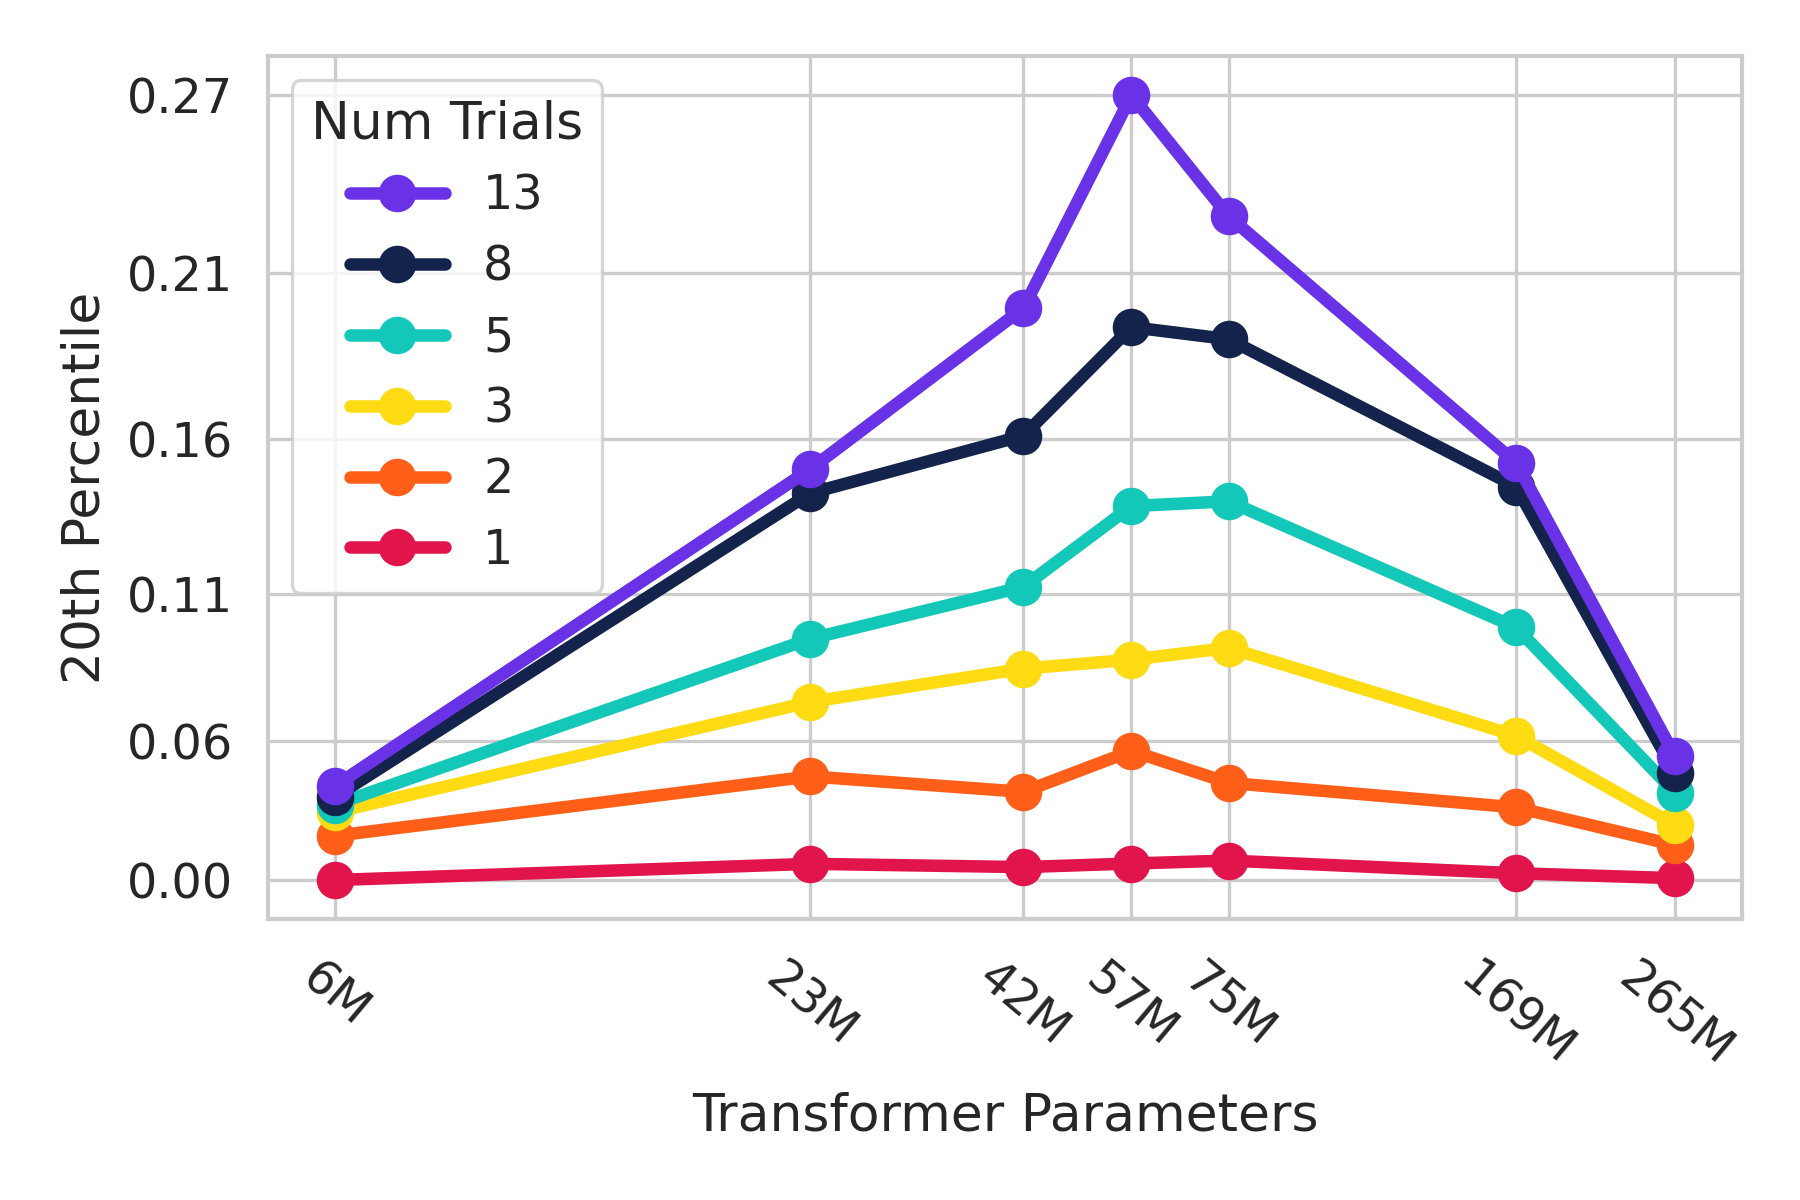
\includegraphics[width=\linewidth]{figures/scaling_flops/parameter_scaling_total_flops_percentile20_log_log.png}
        \vskip -3pt \caption{}
    \label{figure:scaling_parameters_total_flops_20th}
    \end{subfigure}
    \caption{
        Scaling Transformer model size controlling for the total number of FLOPs for the learner and actors, including auto-curriculum evaluation actors.
    \label{figure:scaling_parameters_total_flops}
    }
\end{figure}

\begin{figure}[t!]
    \centering
    \begin{subfigure}[b]{0.49\textwidth}
        \centering
        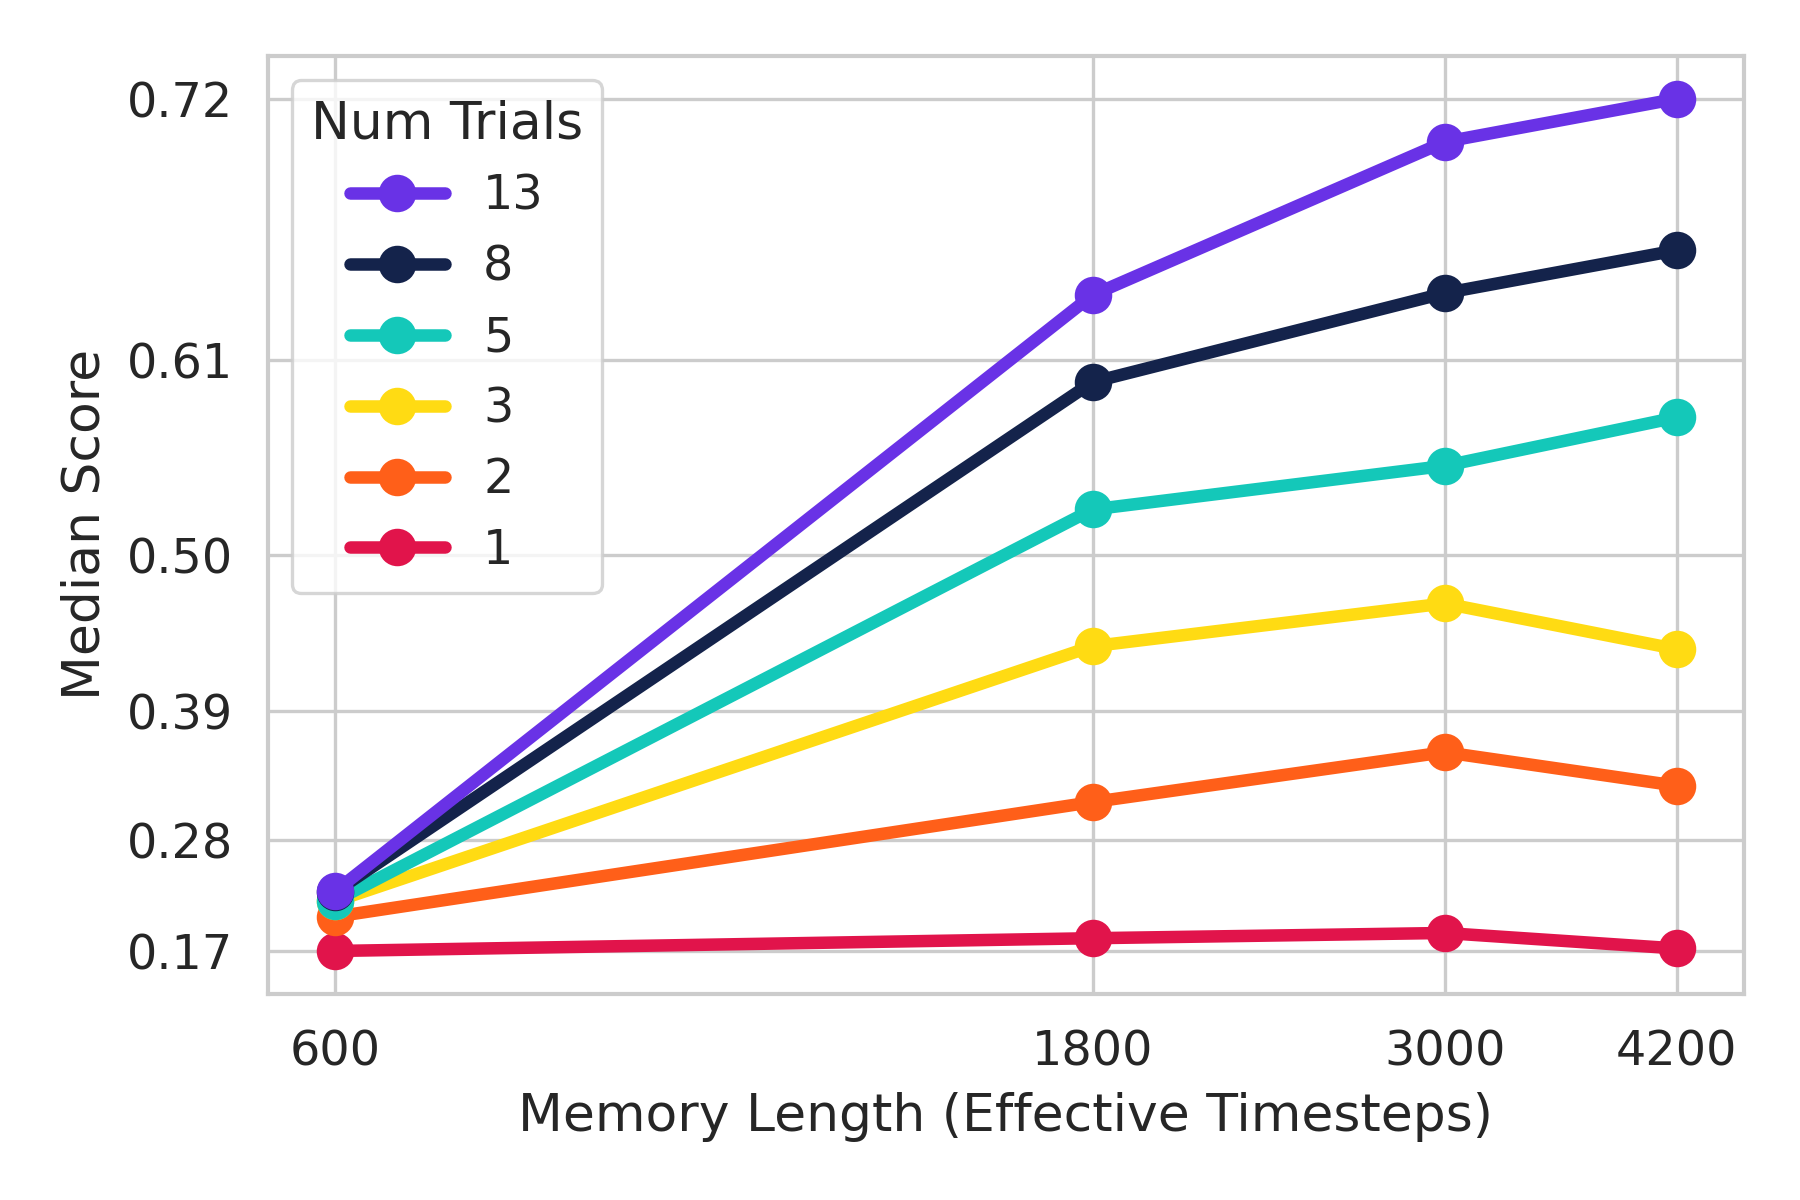
\includegraphics[width=\linewidth]{figures/scaling_flops/memory_scaling_total_flops_percentile50_log_log.png}
        \vskip -3pt \caption{}
    \label{figure:scaling_memory_total_flops_50th}
    \end{subfigure}
    \begin{subfigure}[b]{0.49\textwidth}
        \centering
        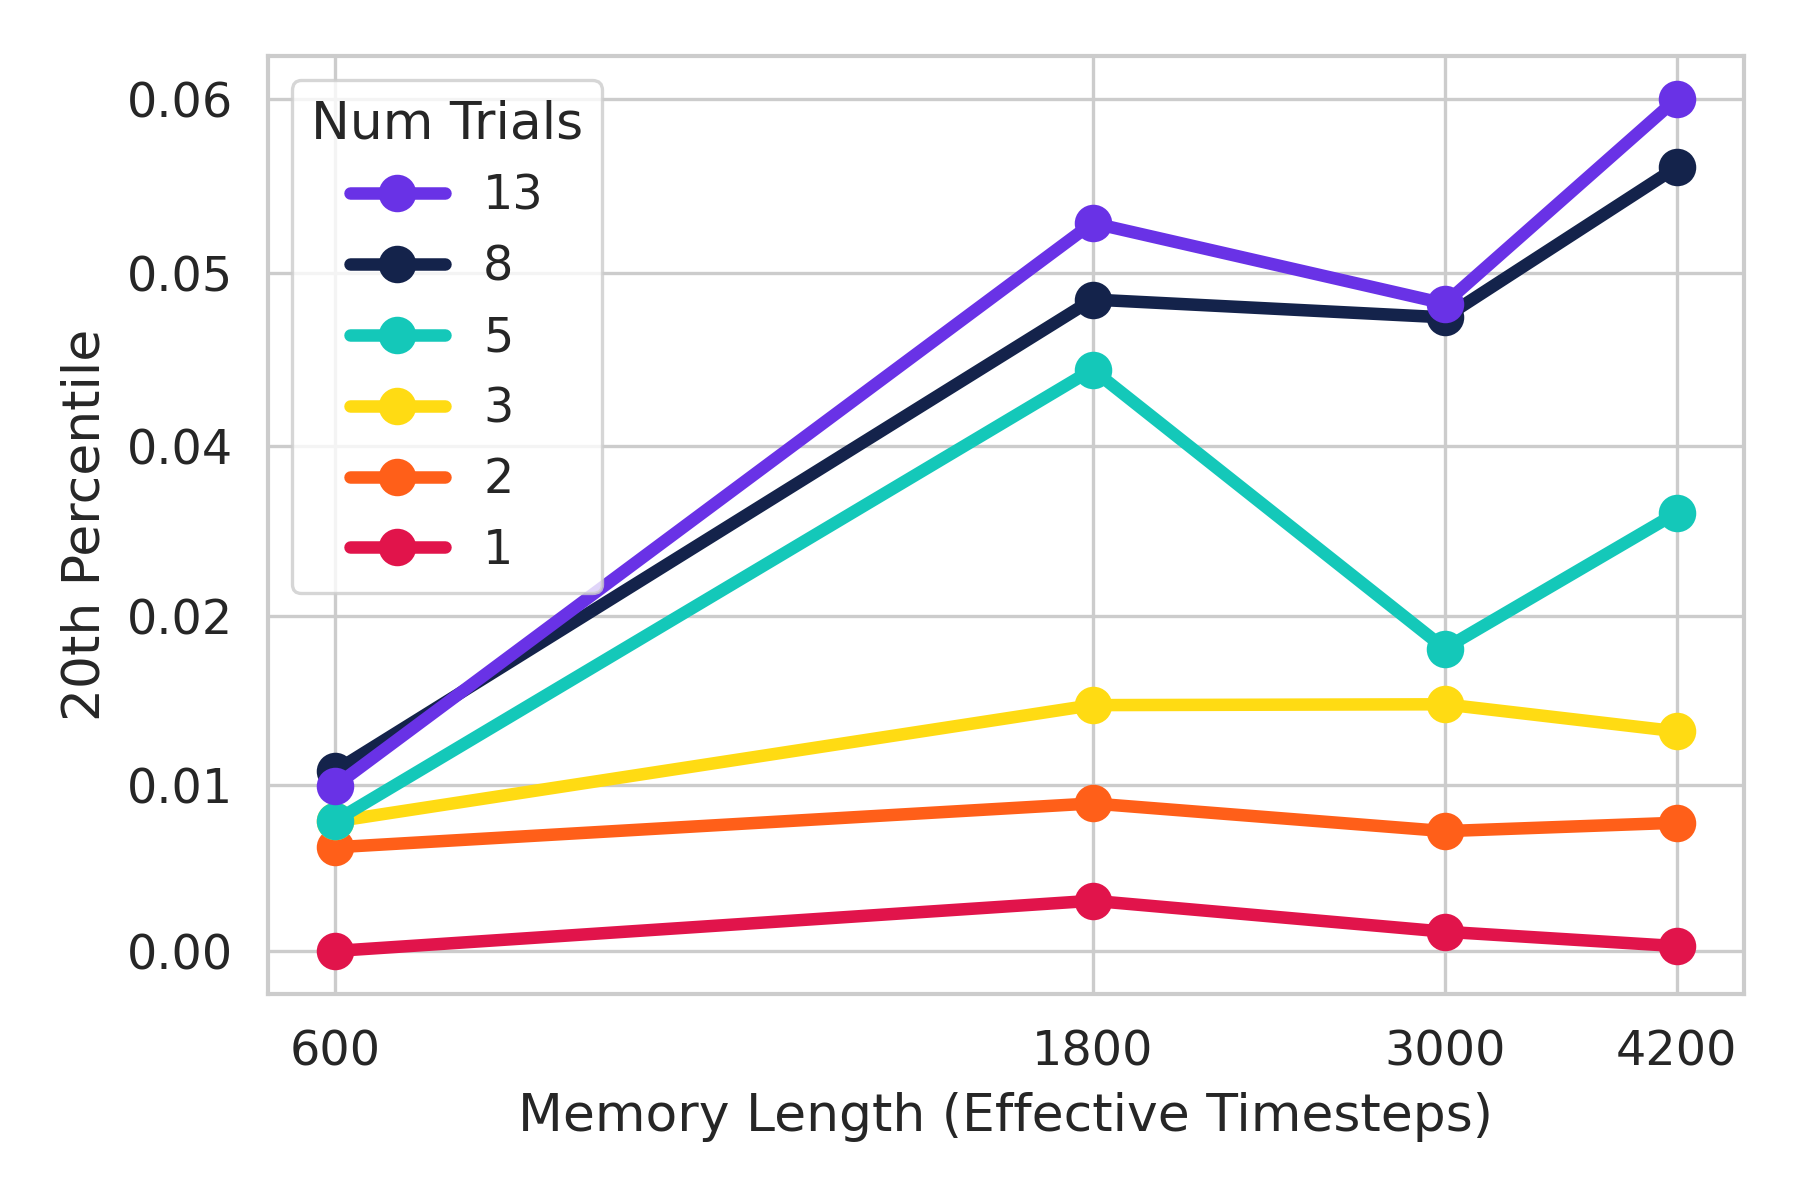
\includegraphics[width=\linewidth]{figures/scaling_flops/memory_scaling_total_flops_percentile20_log_log.png}
        \vskip -3pt \caption{}
    \label{figure:scaling_memory_total_flops_20th}
    \end{subfigure}
    \caption{
        Scaling Transformer-XL memory controlling for the total number of FLOPs for the learner and actors, including auto-curriculum evaluation actors.
    \label{figure:scaling_memory_total_flops}
    }
\end{figure}

\begin{table}[t!]
  \begin{center}
    \caption{FLOPs per frame for different model sizes and memory lengths.}
    \begin{tabular}{c|c|c|c}
    \label{tab:flops}
      Model parameters & Memory & Learner FLOPs per frame & Actor FLOPs per frame \\
      \hline
      6M TXL / 41M total & \multirow{7}{*}{1800} & 1,138,005,632 & 736,987,392\\
      23M TXL / 76M total & & 1,380,255,078 & 2,580,445,440\\
      42M TXL / 112M total & & 1,623,461,663 & 4,489,239,552\\
      57M TXL / 141M total & & 1,821,422,230 & 6,063,742,976\\
      75M TXL / 175M total & & 2,048,253,663 & 7,879,863,808\\
      169M TXL / 353M total & & 3,243,189,525 & 17,560,326,144\\
      265M TXL / 533M total & & 4,443,008,234 & 27,358,181,376\\
      \multirow{3}{*}{23M TXL / 76M total } & 600 & 1,278,491,404 & 963,739,136\\
      & 3000 & 1,481,009,258 & 4,181,042,688\\
      & 4200 & 1,582,270,213 & 5,789,702,144\\
    \end{tabular}
  \end{center}
\end{table}

We multiply the values in Table \ref{tab:flops} by the number of learner/actor steps for each experiment, then,
for a given comparison, we take the largest such value common to all experiments (usually associated with the smallest model) as the total FLOPs, and make the comparison of each model at this number of FLOPs. The results for the FLOPs-matched model scaling experiments are shown in Figure \ref{figure:scaling_parameters_total_flops}. We see a reduction in performance as the model size grows beyond a ``sweet spot'' around 57M Transformer parameters (141M total parameters). Results for the FLOPs-matched memory scaling experiments in Figure \ref{figure:scaling_memory_total_flops} show that there is still benefit to increasing context lengths given a fixed computational budget. Details of the compute used for these experiments can be found in Tables \ref{tab:parameter_scaling_total_flops} (model size) and \ref{tab:memory_scaling_total_flops} (memory).

\begin{figure}[b!]
    \centering
    \begin{subfigure}[b]{0.49\textwidth}
        \centering
        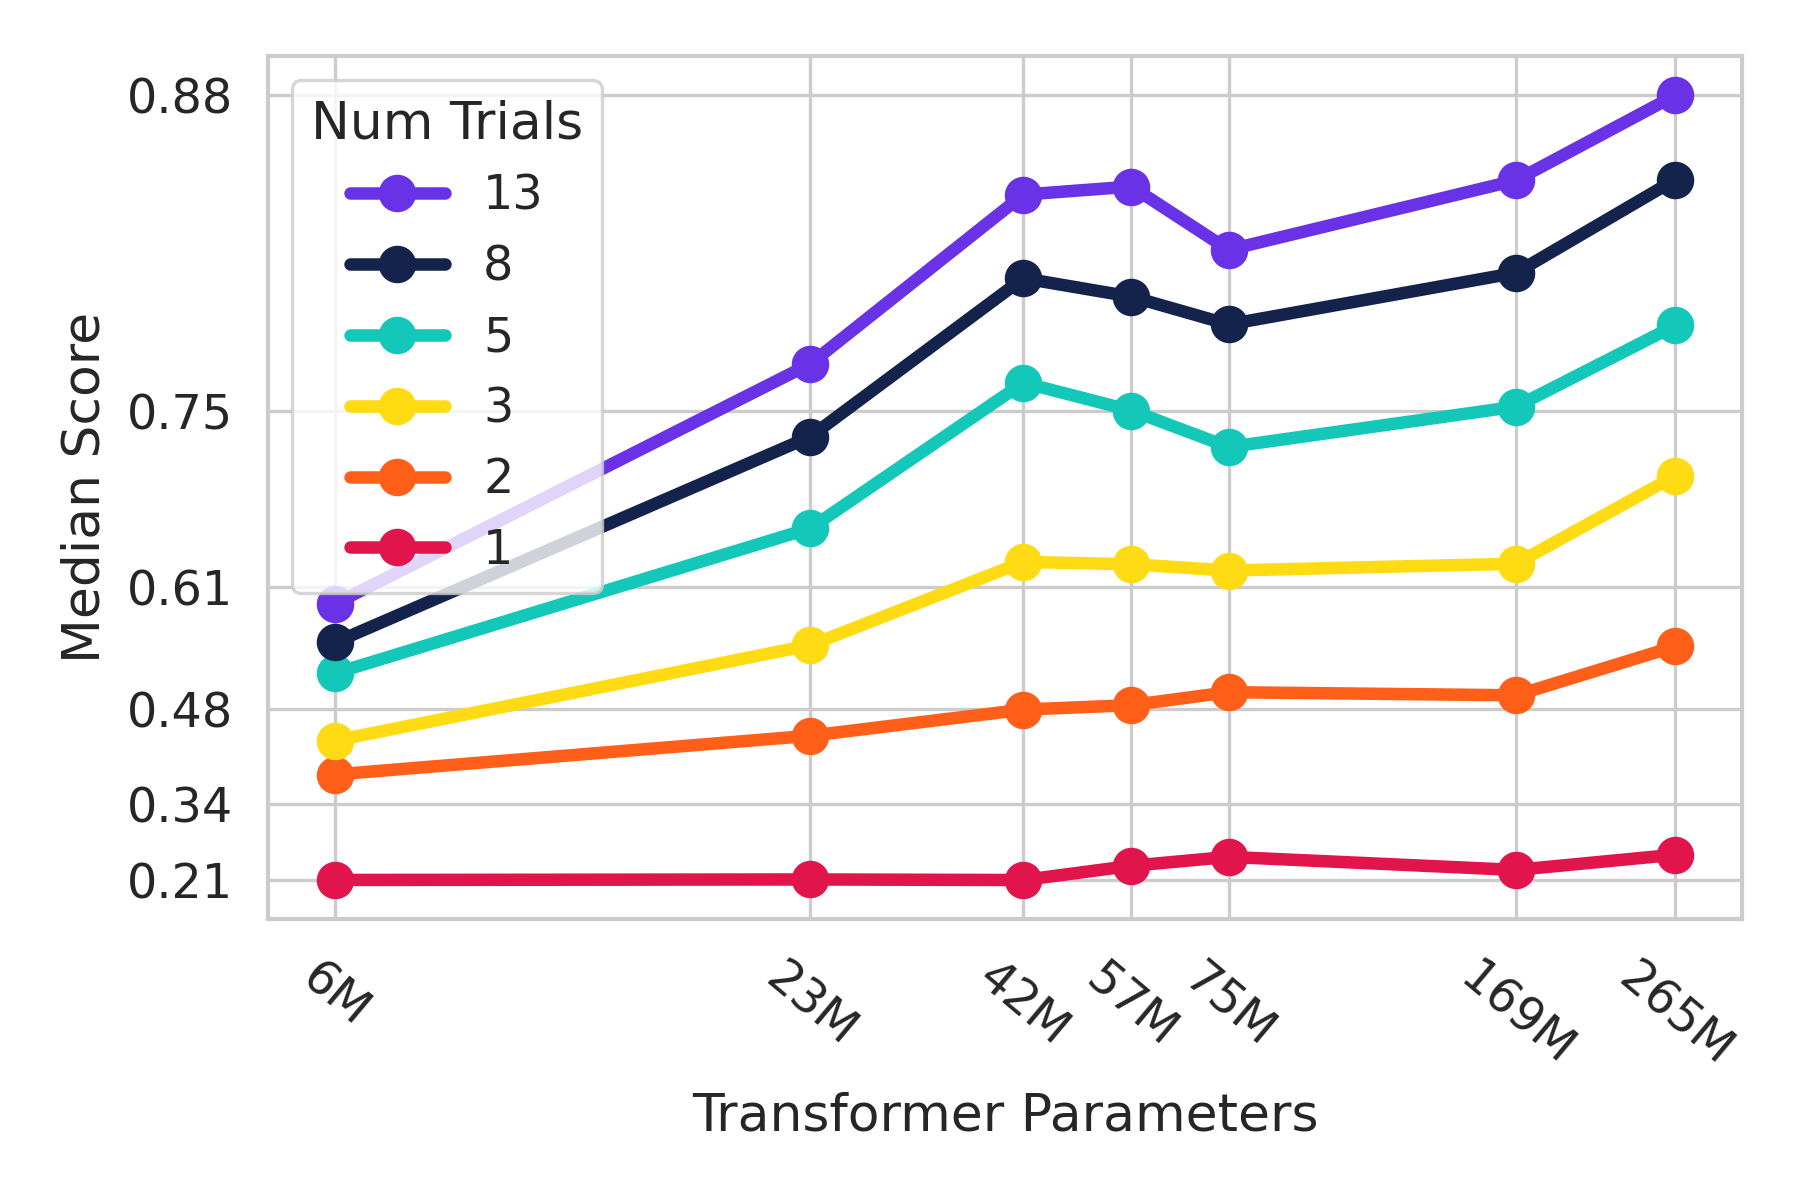
\includegraphics[width=\linewidth]{figures/scaling_flops/parameter_scaling_learner_flops_percentile50_log_log.png}
        \vskip -3pt \caption{}
    \label{figure:scaling_parameters_learner_flops_50th}
    \end{subfigure}
    \begin{subfigure}[b]{0.49\textwidth}
        \centering
        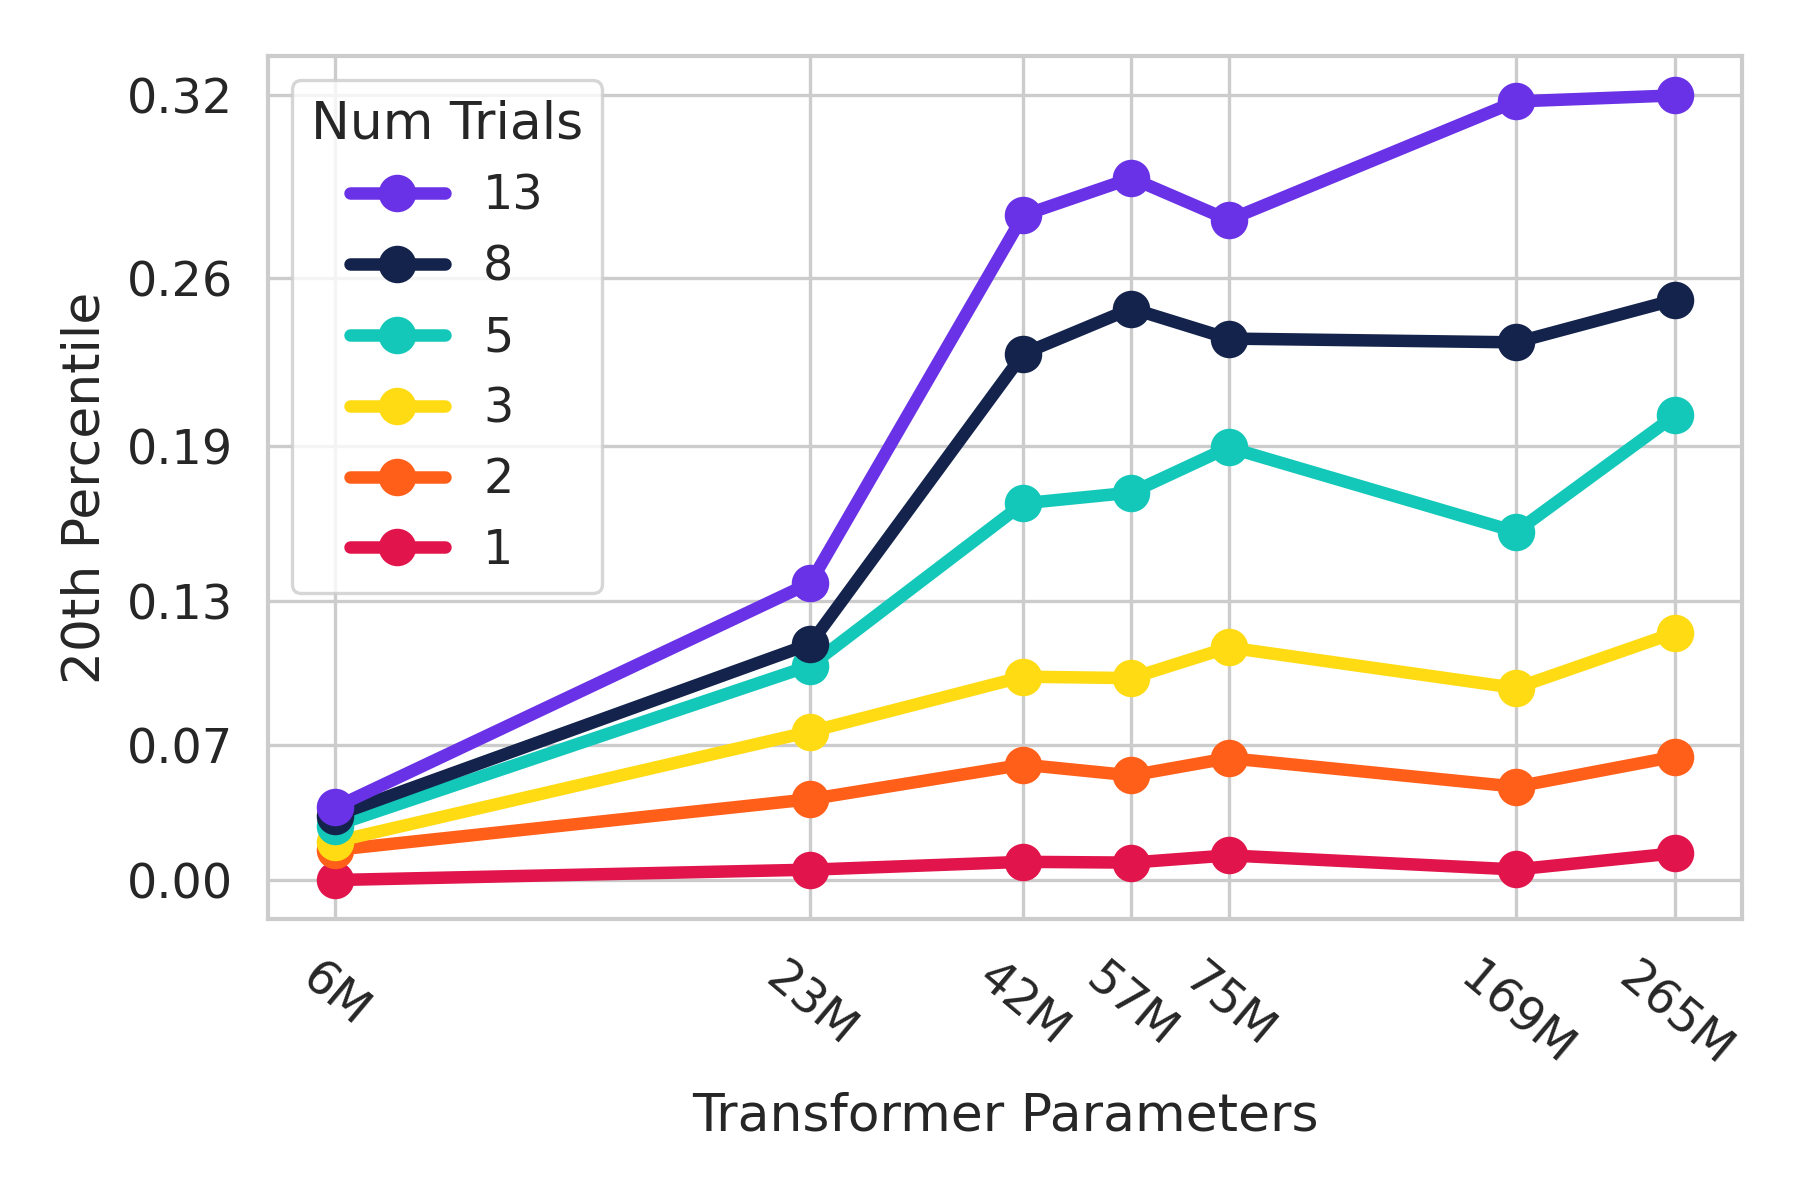
\includegraphics[width=\linewidth]{figures/scaling_flops/parameter_scaling_learner_flops_percentile20_log_log.png}
        \vskip -3pt \caption{}
    \label{figure:scaling_parameters_learner_flops_20th}
    \end{subfigure}
    \caption{
        Scaling Transformer-XL model size controlling for the number of learner FLOPs.
    \label{figure:scaling_parameters_learner_flops}
    }
\end{figure}

\begin{figure}[b!]
    \centering
    \begin{subfigure}[b]{0.49\textwidth}
        \centering
        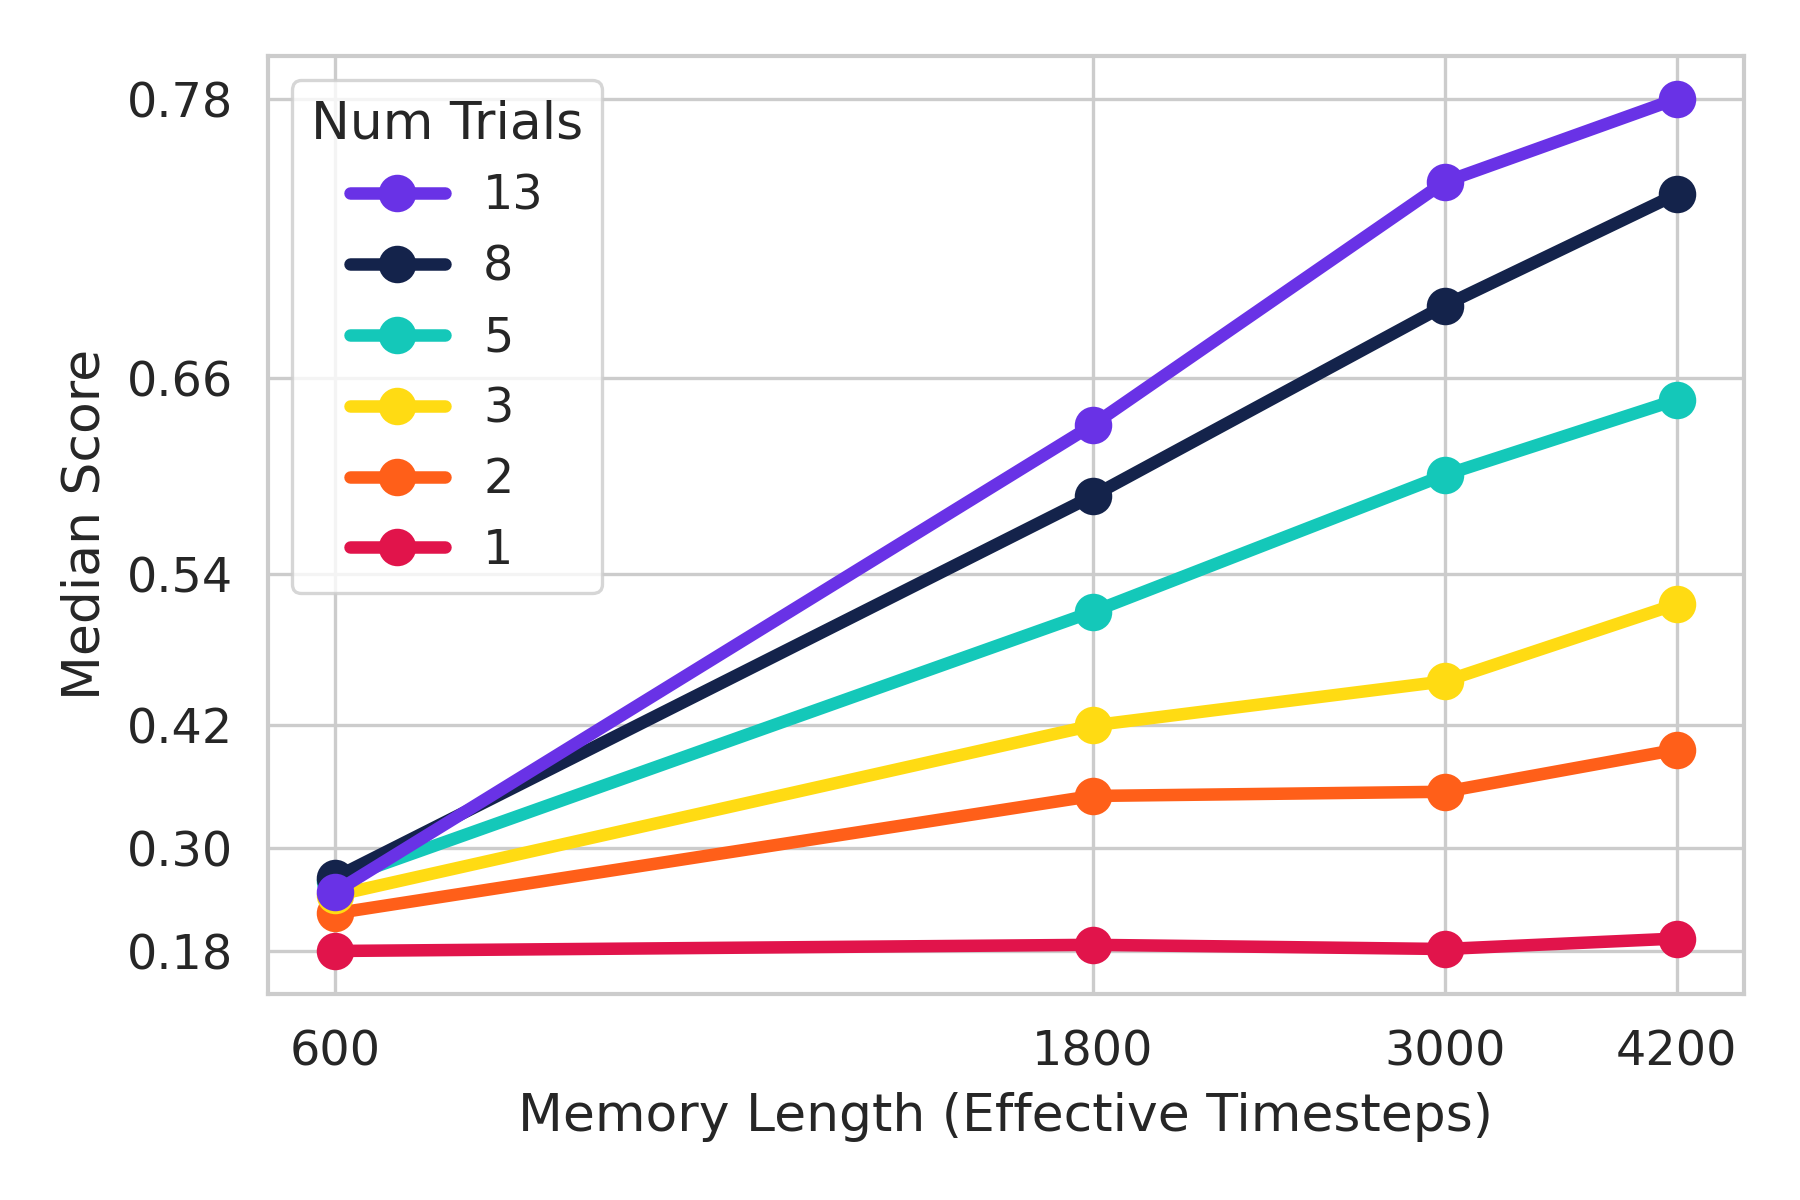
\includegraphics[width=\linewidth]{figures/scaling_flops/memory_scaling_learner_flops_percentile50_log_log.png}
        \vskip -3pt \caption{}
    \label{figure:scaling_memory_learner_flops_50th}
    \end{subfigure}
    \begin{subfigure}[b]{0.49\textwidth}
        \centering
        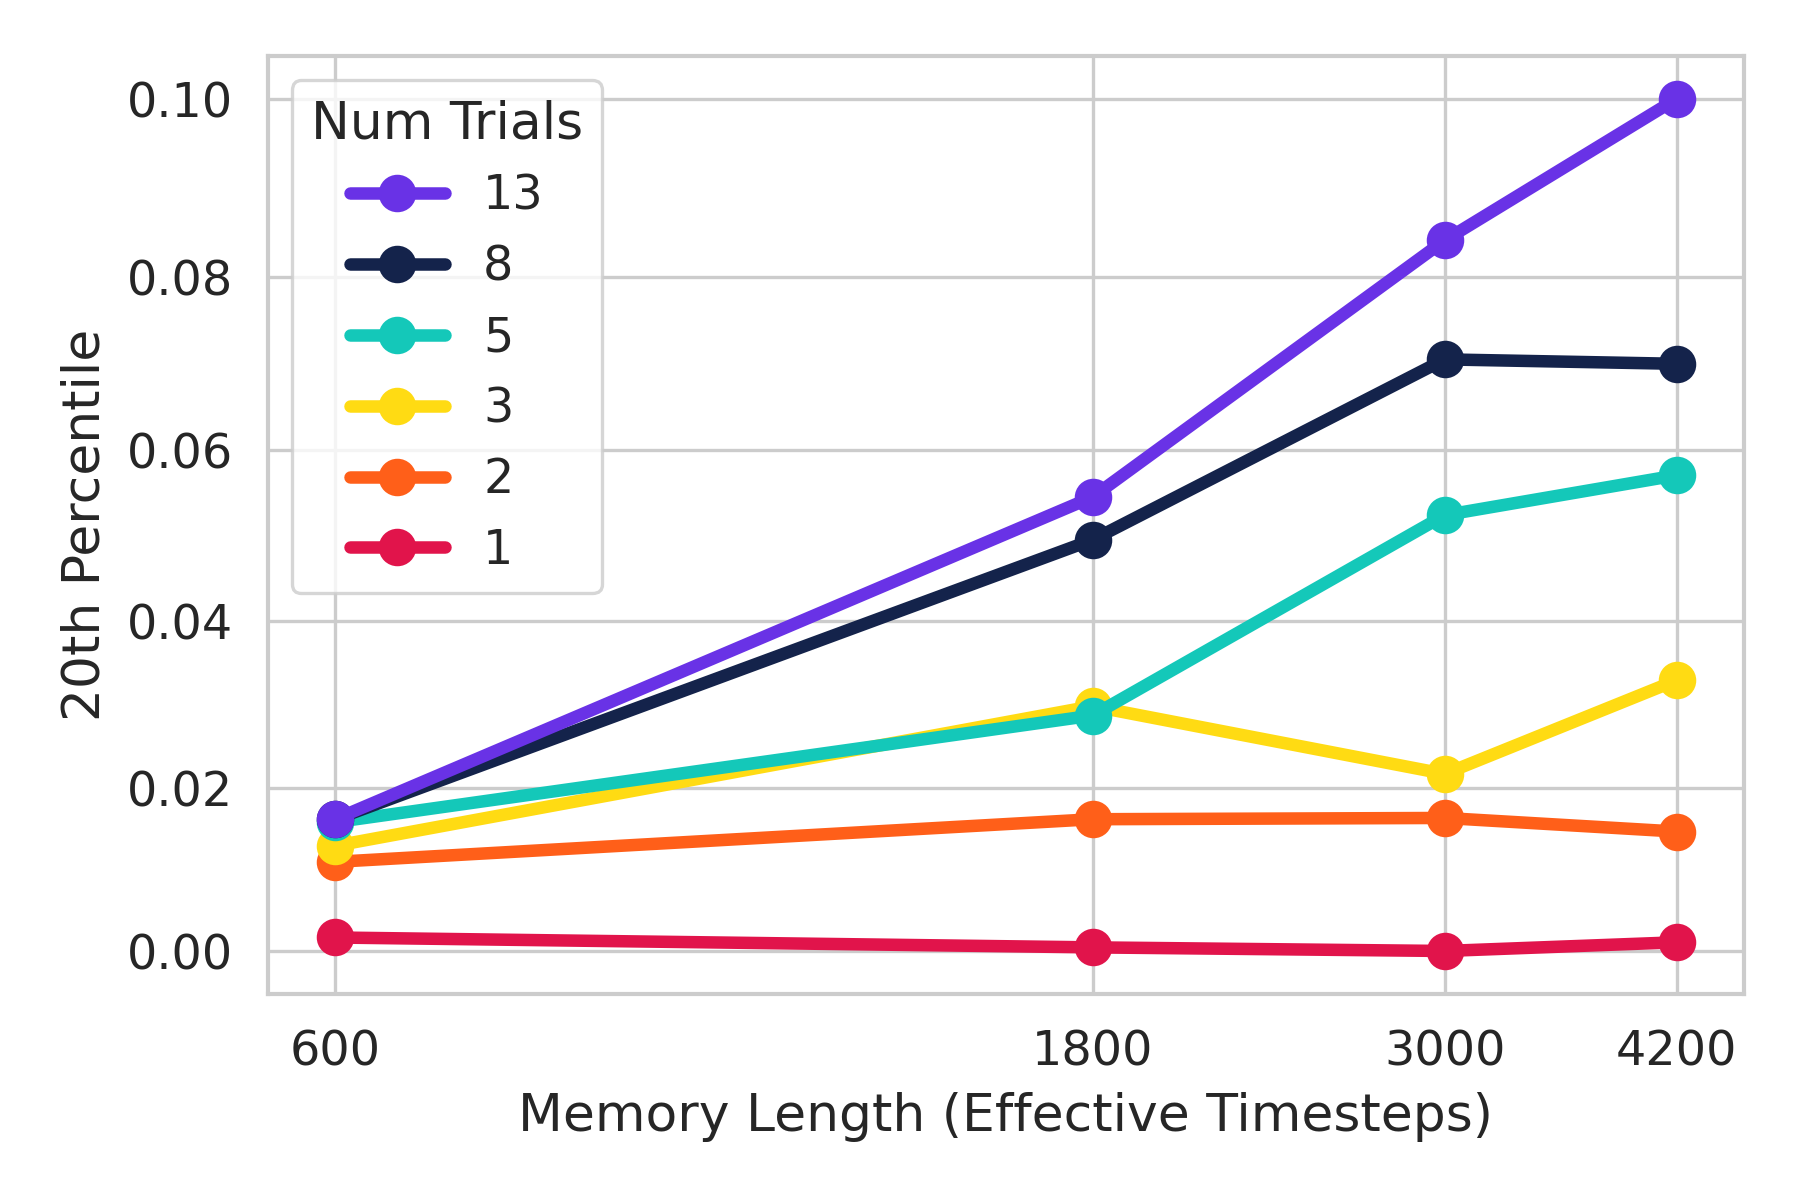
\includegraphics[width=\linewidth]{figures/scaling_flops/memory_scaling_learner_flops_percentile20_log_log.png}
        \vskip -3pt \caption{}
    \label{figure:scaling_memory_learner_flops_20th}
    \end{subfigure}
    \caption{
        Scaling Transformer-XL memory length controlling for the number of learner FLOPs.
    \label{figure:scaling_memory_learner_flops}
    }
\end{figure}

We note that Table \ref{tab:flops} indicates poor scaling of actor step FLOPs with model size, and suspect this could be due to poor optimisation of a single-step query of the Transformer on TPU, compared to the operation batching achieved with a rollout length of 80 on the learner. In order to account for this and for potential discrepancies in number of actor steps due to differences in curriculum evaluation based on model quality, we also provide plots which only account for the learner step FLOPs for each model: Figures  \ref{figure:scaling_parameters_learner_flops} (model size), and \ref{figure:scaling_memory_learner_flops} (memory length). These might be more informative, and show that performance still increases as a function of model size and memory length, albeit not as steeply as when controlling for sample efficiency directly. Details of the compute used for these experiments is shown in Tables \ref{tab:parameter_scaling_learner_flops} (model size) and \ref{tab:memory_scaling_learner_flops} (memory length).

\begin{table}[t!]
  \begin{center}
    \caption{Corresponding learner steps given total FLOPs for each model size.}
    \begin{tabular}{c|c|c|c}
    \label{tab:parameter_scaling_total_flops}
      Model parameters & Memory & Total FLOPs & Learner steps \\
      \hline
      6M TXL / 41M total & \multirow{7}{*}{1800} & \multirow{7}{*}{$2.0 \times 10^{20}$} & 97B\\
      23M TXL / 76M total & & & 44B\\
      42M TXL / 112M total & & & 27B\\
      57M TXL / 141M total & & & 23B\\
      75M TXL / 175M total & & & 18B\\
      169M TXL / 353M total & & & 9B\\
      265M TXL / 533M total & & & 5B\\
    \end{tabular}
  \end{center}
\end{table}

\begin{table}[t!]
  \begin{center}
    \caption{Corresponding learner steps given total FLOPs for each memory length.}
    \begin{tabular}{c|c|c|c}
    \label{tab:memory_scaling_total_flops}
      Model parameters & Memory & Total FLOPs & Learner steps \\
      \hline
      \multirow{4}{*}{23M TXL / 76M total} & 600 & \multirow{4}{*}{$7.9 \times 10^{19}$} & 31B\\
      & 1800 & & 17B\\
      & 3000 & & 11B\\
      & 4200 & & 8B\\
    \end{tabular}
  \end{center}
\end{table}

\begin{table}[t!]
  \begin{center}
    \caption{Corresponding learner steps given learner-step-only FLOPs for each model size.}
    \begin{tabular}{c|c|c|c}
    \label{tab:parameter_scaling_learner_flops}
      Model parameters & Memory & Learner step FLOPs & Learner steps \\
      \hline
      6M TXL / 41M total & \multirow{7}{*}{1800} & \multirow{7}{*}{$1.0 \times 10^{20}$}& 92B\\
      23M TXL / 76M total & & & 76B\\
      42M TXL / 112M total & & & 65B\\
      57M TXL / 141M total & & & 58B\\
      75M TXL / 175M total & & & 51B\\
      169M TXL / 353M total & & & 32B\\
      265M TXL / 533M total & & & 23B\\
    \end{tabular}
  \end{center}
\end{table}

\begin{table}[t!]
  \begin{center}
    \caption{Corresponding learner steps given learner-step-only FLOPs for each memory length.}
    \begin{tabular}{c|c|c|c}
    \label{tab:memory_scaling_learner_flops}
      Model parameters & Memory & Learner step FLOPs & Learner steps \\
      \hline
      \multirow{4}{*}{23M TXL / 76M total} & 600 & \multirow{4}{*}{$3.9 \times 10^{19}$} & 39B\\
      & 1800 & & 36B\\
      & 3000 & & 29B\\
      & 4200 & & 25B\\
    \end{tabular}
  \end{center}
\end{table}

